\chapter{Forschungsproblem und Forschungsziel}
\label{kap:forschungsproblem_forschungsziel}
Schweizer fahren gerne Zug, dies zeigt ein Artikel von Litra, welcher die Nutzung des Zuges in Europa untersucht untersuchte \parencite{litra_bahnfahrtstatistik_europa_2023}. Alleine im Jahr 2023 legten die Schweizer rund 2'466 Bahnkilometer pro Einwohner zurück (siehe Abbildung \ref{fig_schweizer_fahren_zug}. Dies entspricht einem Zuwachs von rund 13 Prozent im Vergleich zum Vorjahr. 

\begin{figure}[H]
    \caption{Zurückgelegte Kilometer pro Einwohnerin und Einwohner 2023 (Personenkilometer) \parencite{litra_bahnfahrtstatistik_europa_2023}}
    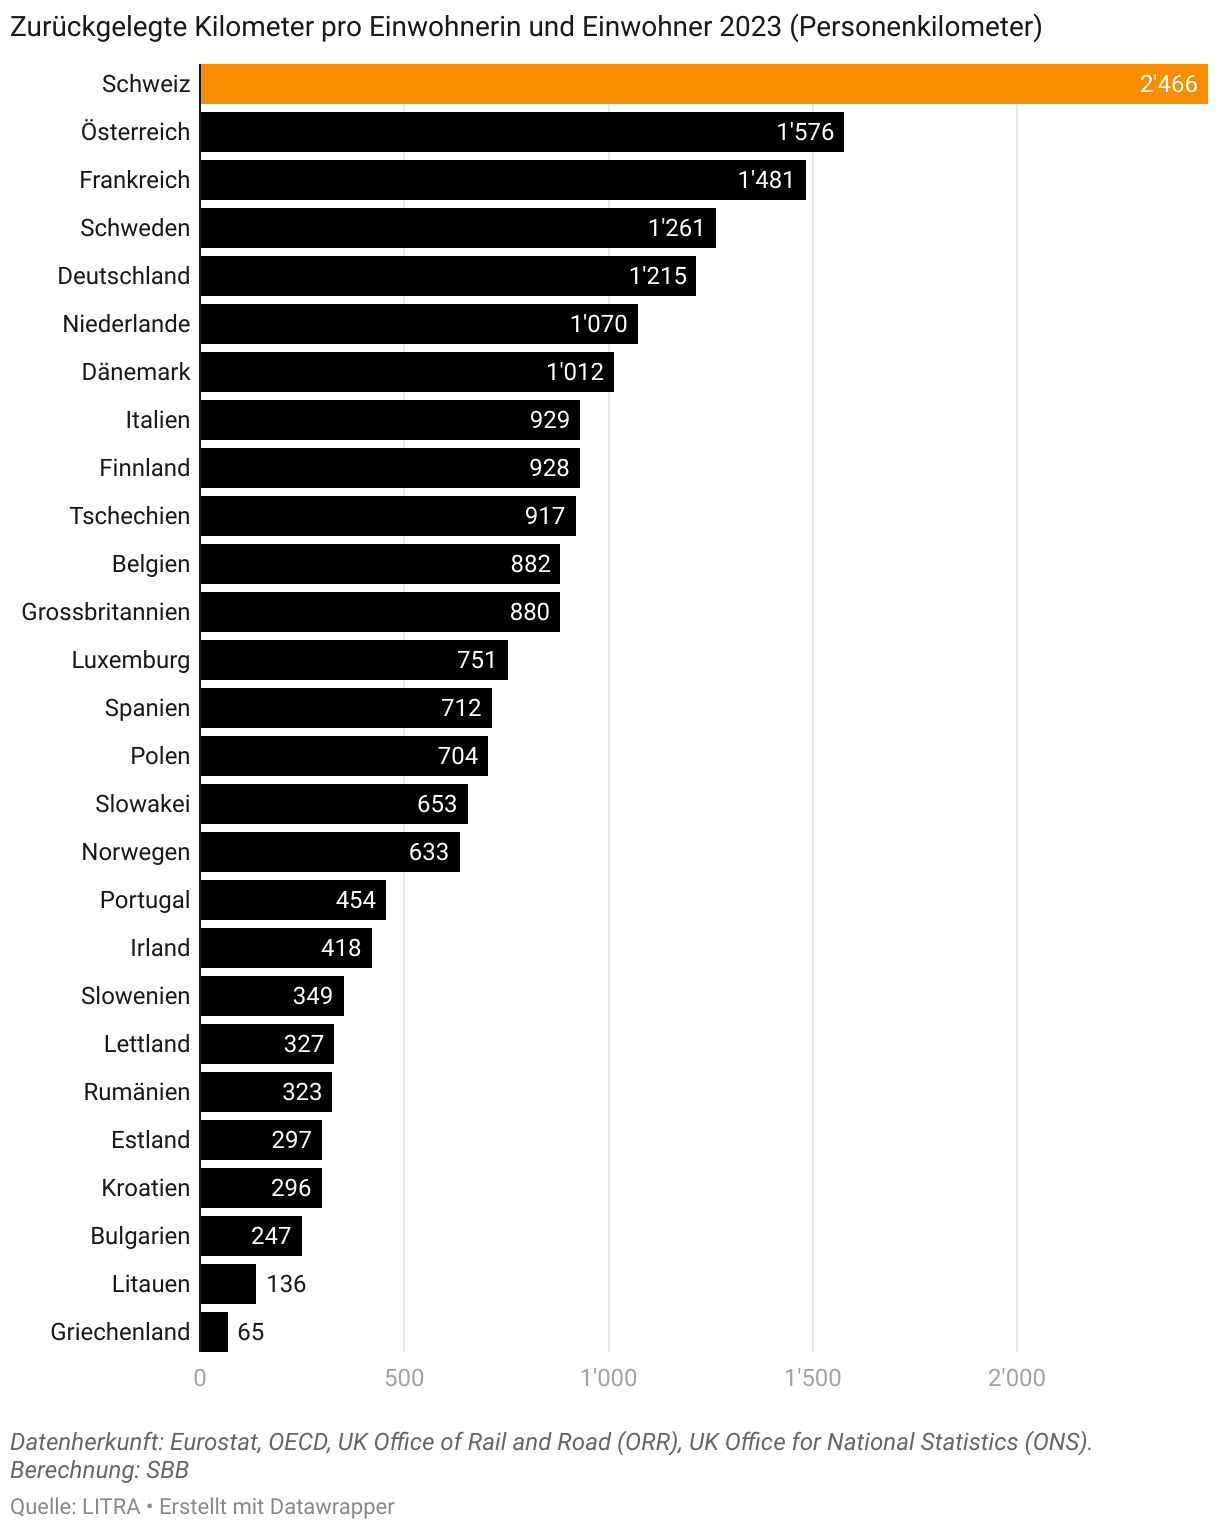
\includegraphics[height=10cm]{content/00_assets/schweizer_fahren_zug.png}
    \label{fig_schweizer_fahren_zug}
\end{figure}

Auch scheint es keine Anzeichen einer Abschwächung der Zugnutzung zu geben, ganz im Gegenteil. Gemäss der \acrfull{sbb} sollen im Jahr 2040 bereits zwei Millionen Menschen pro Tag mit dem Zug fahren, dies entspricht einer Zunahme von rund 30 Prozent \parencite{sbb_ausbauschritt_2025}.

Schaut man sich die Zahlen und Fakten für das SBB-Zugverkehrsnetz aus dem Jahr 2024 an, ergeben sich auch beachtliche Werte. Täglich werden rund 1.4 Millionen Menschen mithilfe von 11'569 Zügen transportiert. Um das Zugnetz der SBB auf Stand zu halten, werden rund 20'000 Baustellen pro Jahr betrieben. Um es mit den Worten der SBB auszudrücken, ist Bauen und Fahren eine Herausforderung \parencite[S.8 - 9]{sbb_geschäftsbericht_2024}. Jedoch ist insbesondere das Fahren nicht nur eine Herausforderung für die Zugnetzbetreiber, sondern auch für die Passagiere, primär dann, wenn Verspätungen involviert sind.

Die vorliegende Arbeit hat sich daher zum Ziel gesetzt, visuelle Muster und Anomalien im SBB-Zugverkehrsnetz zu analysieren. Hierzu soll ein webbasiertes Visual-Analytics-Tool entworfen werden. Im Fokus der Arbeit stehen hierbei primär Zugverspätungen.

